\section{Effective Strain Calibration}

For strain coefficient calibration we assume idealized basins with  different materials including a rock half space, dense sediment and loose sediment inside the basin. We only allow the materials inside the basin to behave nonlinear or equivalent linear.  In the first attempt we assume that only shear strains are dominant and effective. Therefore, we use the following equation.

 \begin{equation}
 \gamma_{max} = G(A \gamma_{xy}^{2} + B\gamma_{xz}^{2} + C\gamma_{yz}^{2} )^H
 \end{equation}


 We use a point source model with seismic moment corresponding to $Mw=4.5$. Fig.~\ref{fig:study_region} show the basin, epicenter, and stations location. 

\begin{figure}[H]
    \centering
    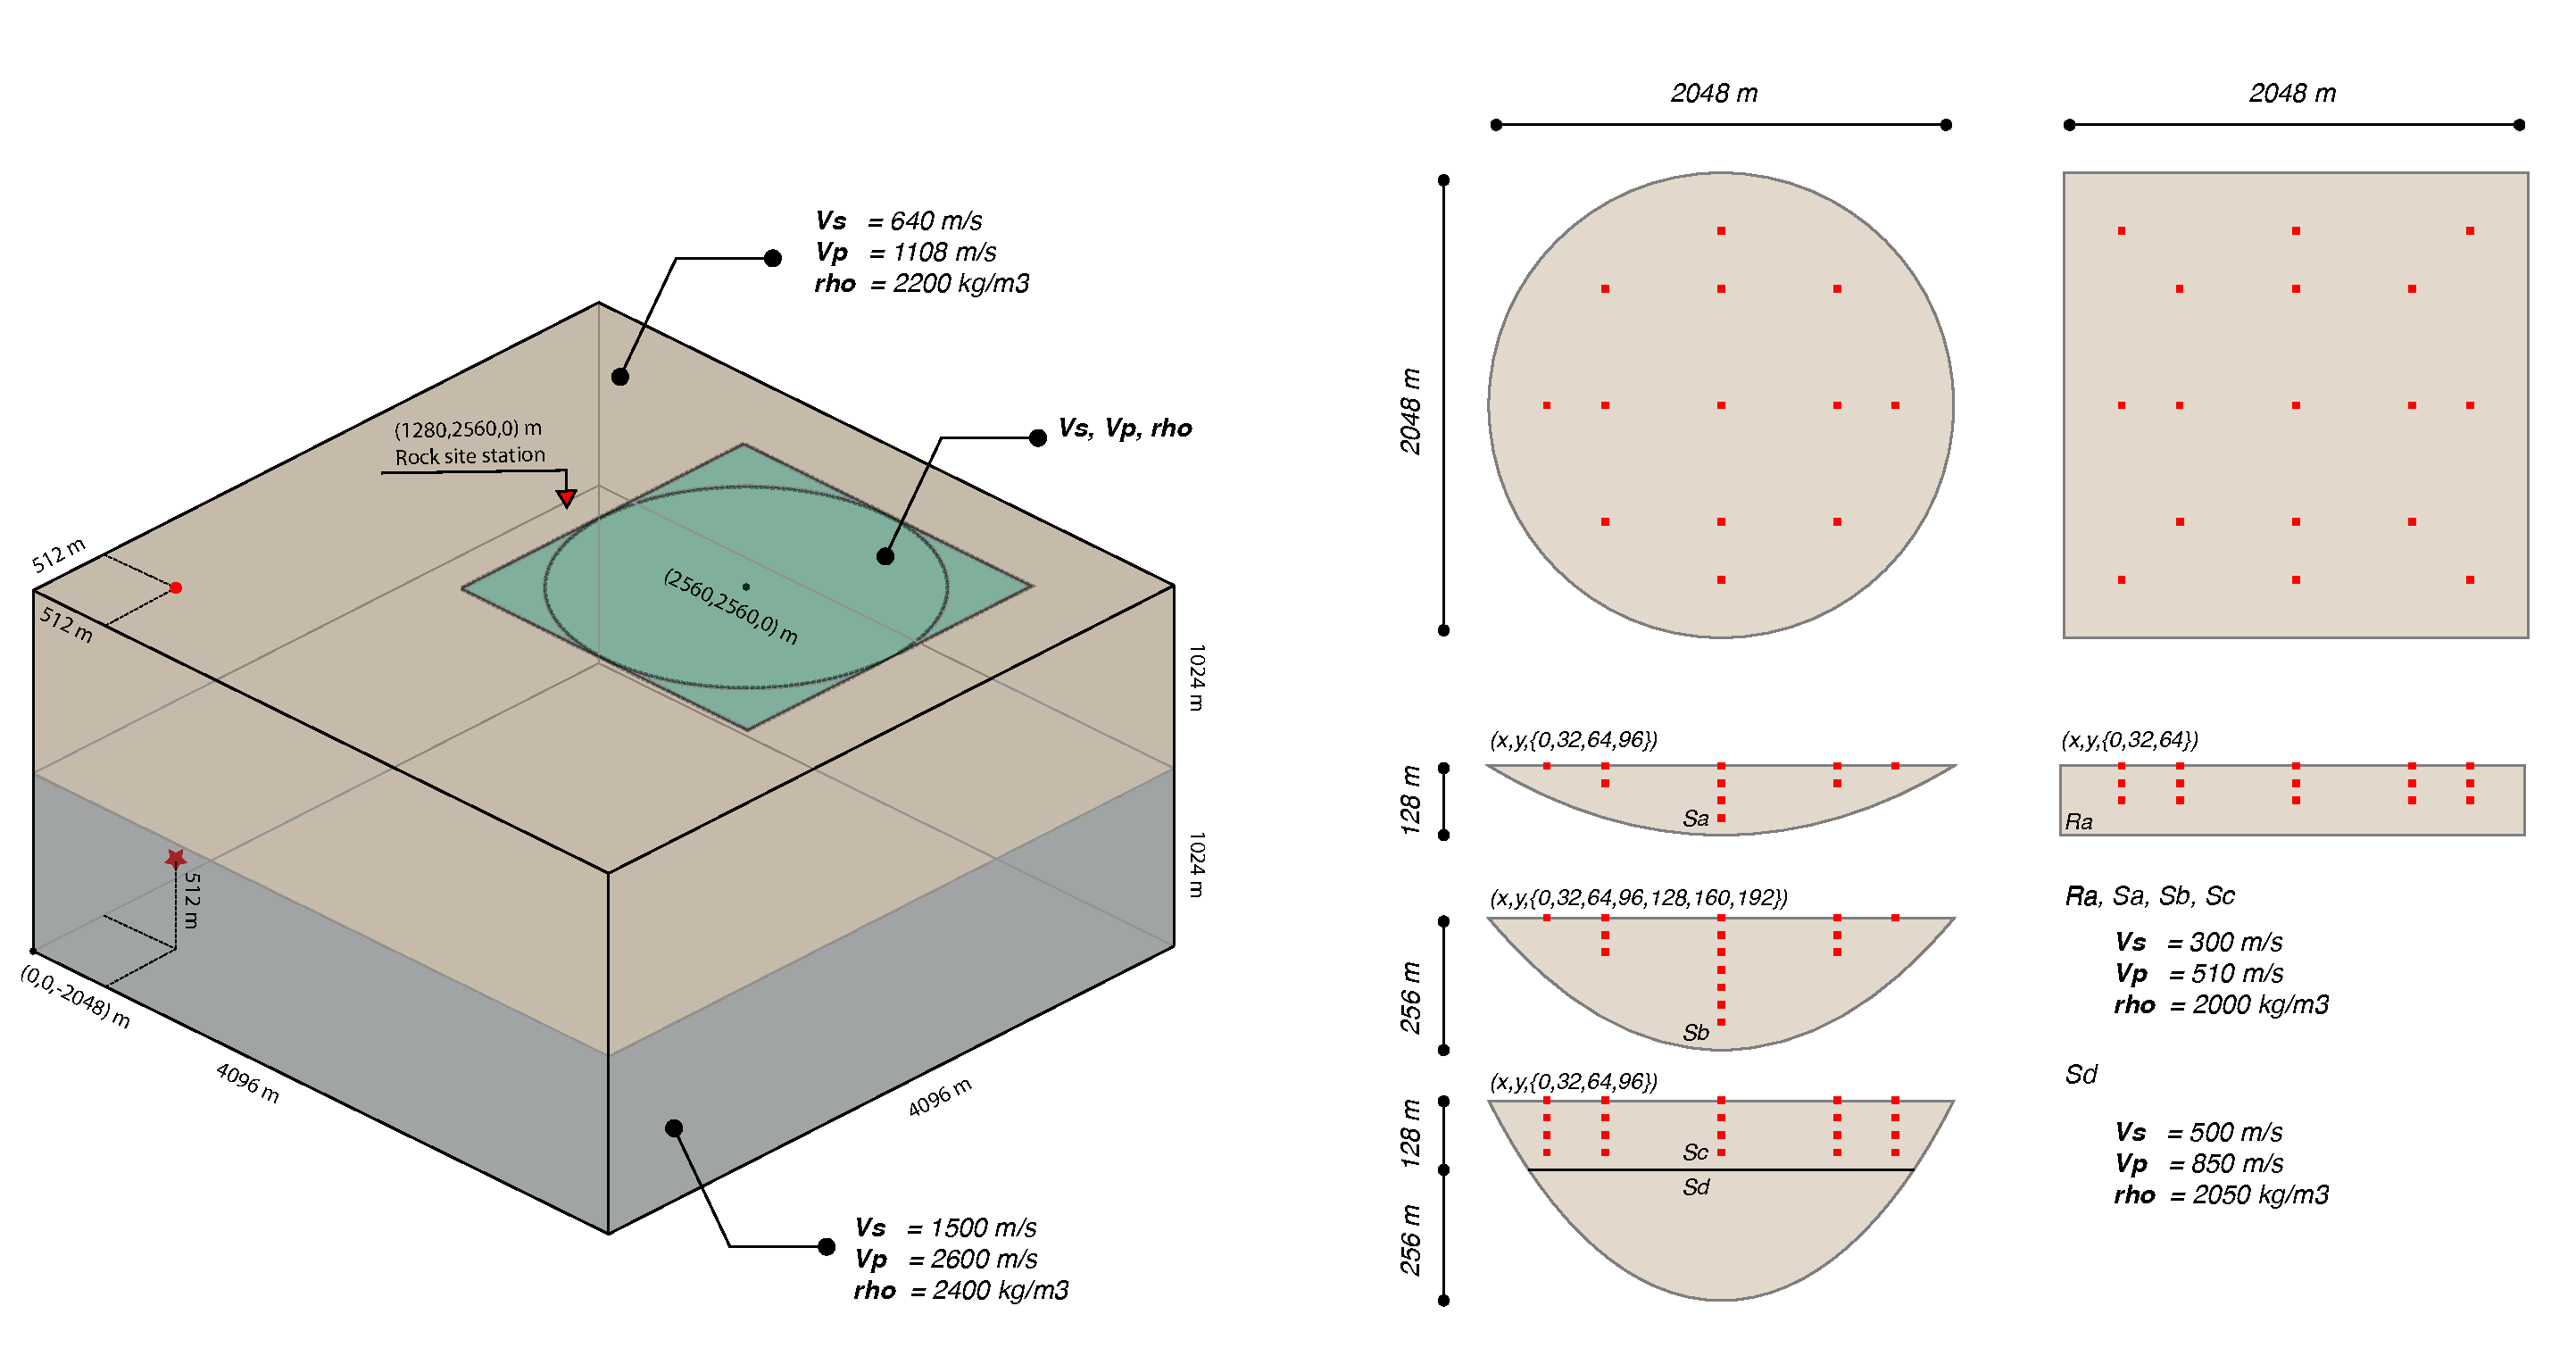
\includegraphics[width=\textwidth]{figures/pdf/study_region.pdf}
    \caption{Idealized basins for effective strain calibration}
    \label{fig:study_region}
\end{figure}


\subsection{Nonlinear Simulation}

Equivalent linear method is an approach to approximate the fully nonlinear method. The damping and shear modulus reduction curve with respect to strain are two extra inputs for adding to linear simulation to conduct equivalent linear method. In this study, in order to make sure that the calibration of the effective strain level based on comparing the results with fully nonlinear simulation. The fully nonlinear simulation, which is used in this study, is based on vonMises model with Modified Frederich-Armstrong formulation. We extract the shear modulus reduction and damping curve for the model and use it as an input values in the equivalent linear model. 

\subsubsection{von Mises Modified Frederich-Armstrong formulation}

For nonlinear constitutive model we use Modified Frederich-Armstrong formulation. No elastic region is considered, thus Gamma=0. The modification generates closed hysteric loops.

\subsubsection{Shear Modulus degradation and Damping}

We numerically extracted shear modulus degradation and damping curves from von Mises Modified Frederich-Armstrong formulation for the following soil materials:

\begin{itemize}
\item Elastic limit (k) = 0
\item Undrained strength (Su) = 70 $KN$
\item Material parameter to adjust (psi) = 100
\item S-wave velocity (Vs) = 300 $m/s$
\item Poisson's ration ($\mu$)=0.3
\item Density ($\rho$) = 2000 $kg/m^3$
\end{itemize}

Fig.~\ref{fig:GD_18_points_FAM_su70kn_psi100_vs300} shows the shear modulus degradation and damping curve. 

 \begin{figure}[H]
    \centering
    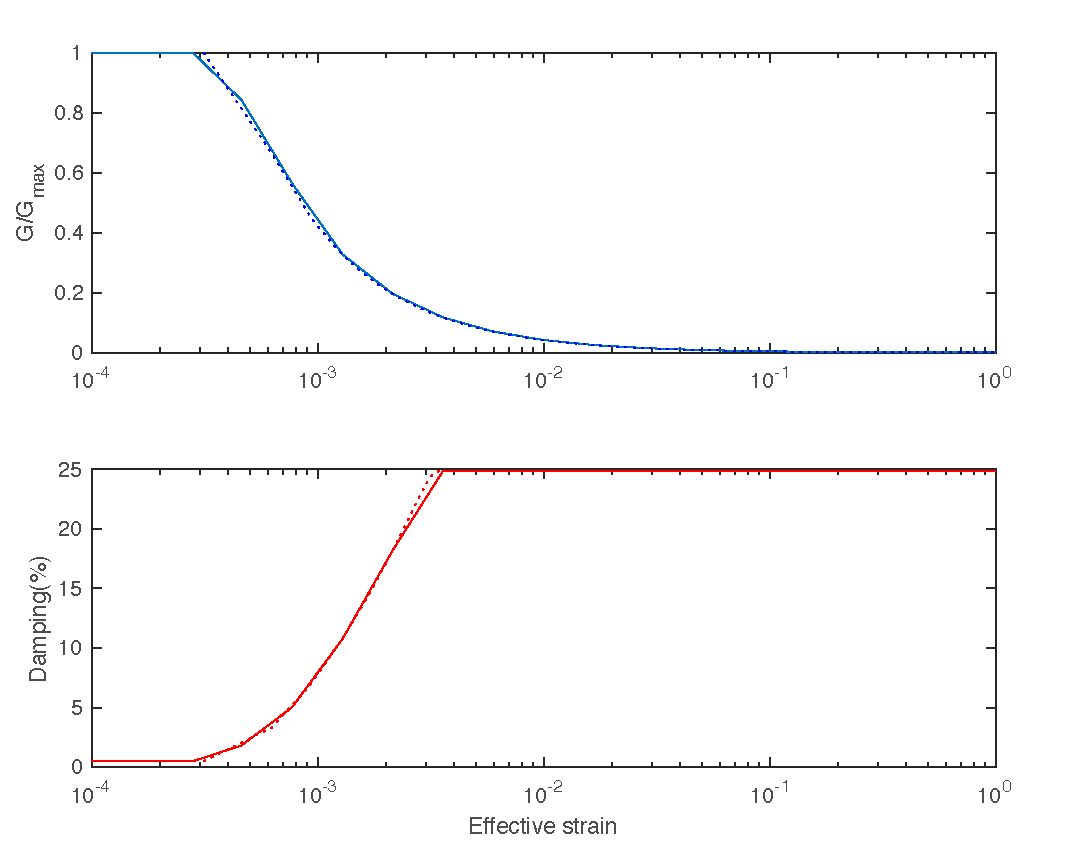
\includegraphics[width=300px]{figures/pdf/GD_18_points_FAM_su70kn_psi100_vs300.pdf}
    \caption{Variation of shear modulus and damping for the study soil material with based on effective strain level. Dashed-line is the original value based on 4000 numerical values. The solid line represents the interpolated values for 18 points.}
    \label{fig:GD_18_points_FAM_su70kn_psi100_vs300}
\end{figure}

%% source model

\subsection{Source Model}

In this study, in order to calibrate the nonlinear simulation and equivalent simulation we used a point source. In order to reduce the effect of permanent displacement at the final results we defined the source slip function as a combination of Ricker pulses. Fig.~\ref{fig:slip_function} represent the source slip function. 

 \begin{figure}
    \centering
    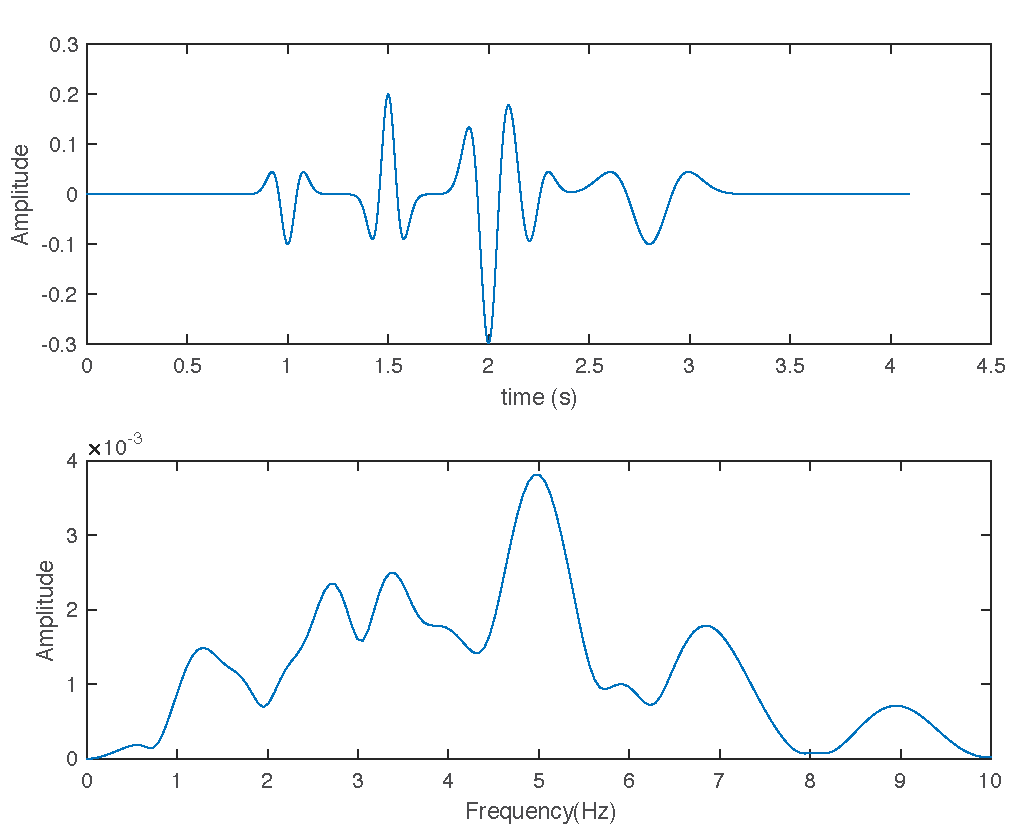
\includegraphics[width=300px]{figures/pdf/slip_function.pdf}
    \caption{Point source slip function}
    \label{fig:slip_function}
\end{figure}









